%----------------------------------------------------------------------------------------
%	Inställningar och dokumentkonfiguration
%----------------------------------------------------------------------------------------

\documentclass[paper=a4, fontsize=11pt]{report} % A4-sida och 11 punkters fontstorlek

\usepackage[T1]{fontenc} % 8-bitarskodning som har 256 glyfer
\usepackage[swedish]{babel} % Svenskt språk
\usepackage[utf8]{inputenc} % För svenska tecken
\usepackage{dtklogos} % Logos
\usepackage{wallpaper} % Bakgrundsbild
\usepackage{fancyhdr} % Specialsidhuvud och sidfot
\usepackage{enumerate} 
\usepackage{hyperref}
\usepackage{textcomp}
\usepackage{xifthen}% provides \isempty test
\pagestyle{fancyplain} % Använd sidhuvud och sidfot på alla sidor
\fancyhead[L]{Laboration 1 -- 1DV416 -- HT13 -- Windowsadministraion I} % Titel till vänster i sidhuvud
\fancyhead[C]{} % Tomt i mitten
\fancyhead[R]{} % Tomt till höger
\fancyfoot[L]{{\color{gray}\textcopyright \ 2013 Jacob Lindehoff}} % Tomt till vänster
\fancyfoot[C]{}  % Tomt i mitten
\fancyfoot[R]{\thepage} % Sidnumrering till höger i sidfoten
\renewcommand\thesection{\arabic{section}} % Section beter sig som i dokumentklassen article

\newcommand{\win}[1]{Microsoft Windows Server\ifthenelse{\isempty{#1}}{}{ #1}}
\newcommand{\gui}[0]{``Server with a GUI''}
\newcommand{\core}[0]{Windows Server Core}
%----------------------------------------------------------------------------------------
%	TITLE SECTION
%----------------------------------------------------------------------------------------
\newcommand\BackgroundPic{
    \put(-50,-50){
    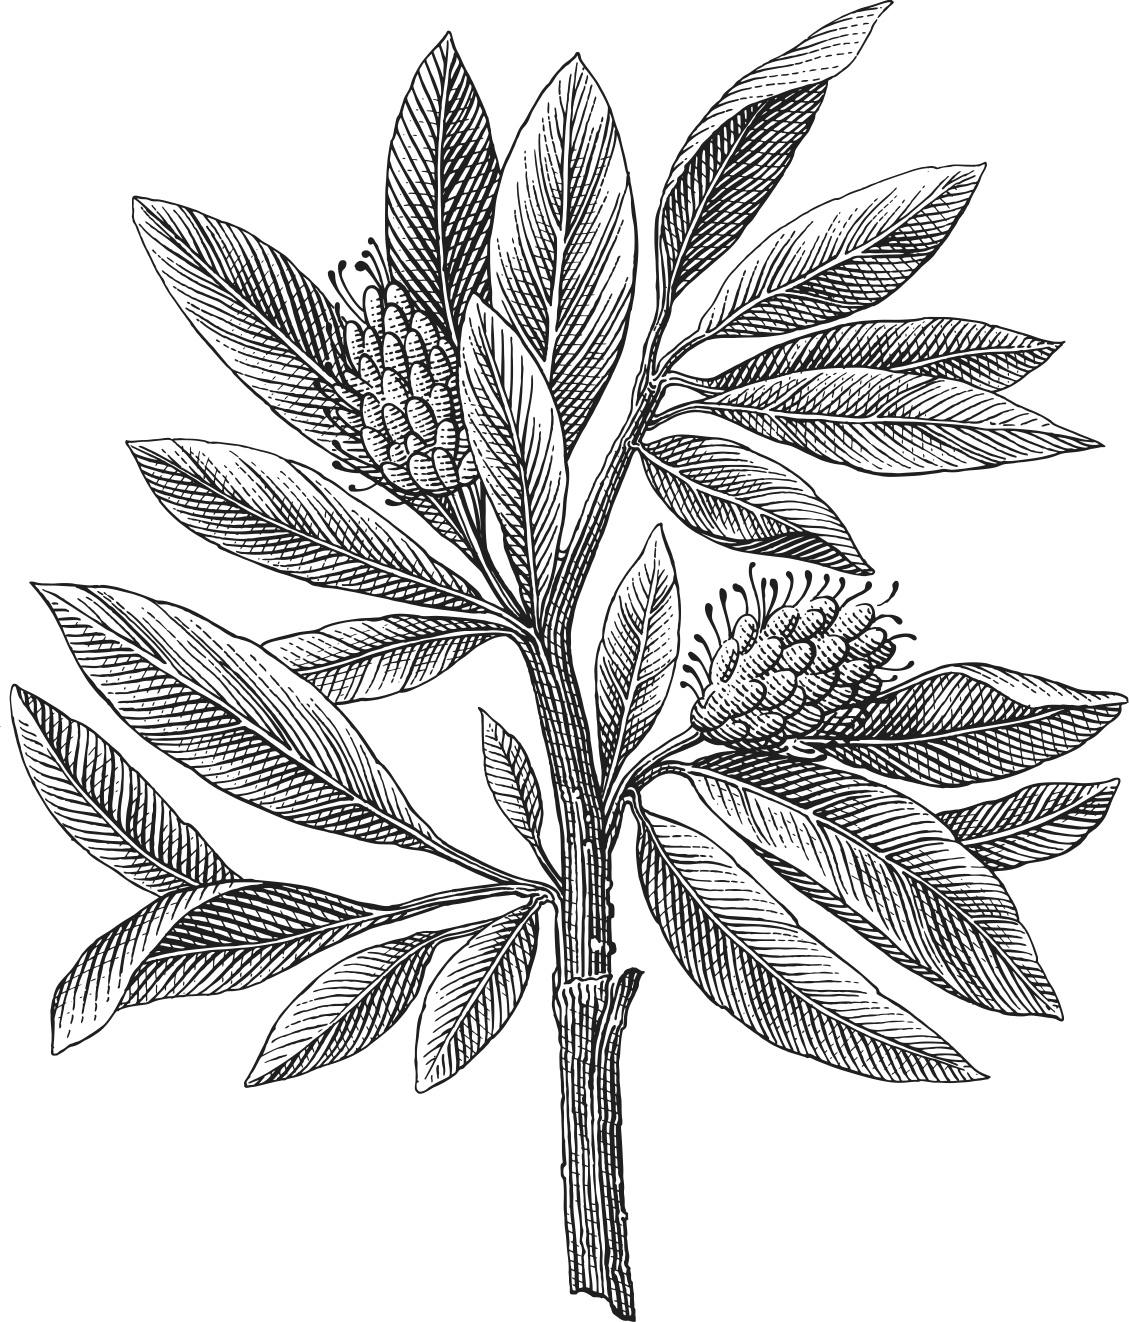
\includegraphics[keepaspectratio,scale=0.65]{lnu_etch.png} % Bakgrundsbild
    }
}
\newcommand\BackgroundPicLogo{
    \put(15,700){
    
\includegraphics[keepaspectratio,scale=0.10]{logo.png} % Logga i vänstra hörnet
    }
}

\newcommand{\horrule}[1]{\rule{\linewidth}{#1}} % Skapa hortisontell linje

\title{	\vspace{-10cm}
    \normalfont \normalsize
    \textsc{Linnéuniversitetet} \\ [25pt] % Universitetes namn
    \horrule{0.5pt} \\[0.4cm] % Tunn linje högst upp
    \huge Laboration 1\\ % Arbetes titel
	\large \textcolor{gray}{1DV416 -- Windowsadministraion I}
    \horrule{0.5pt} \\[0.4cm] % Tunn linje längst ner
}

% \author{Jacob Lindehoff} % Författarnas namn

\date{\normalsize\today} % Dagens datum

\begin{document}
\AddToShipoutPicture*{\BackgroundPic} % Lägger in backgrundsbild på första sidan
\AddToShipoutPicture*{\BackgroundPicLogo}
\maketitle % Skriv ut titeln
\noindent % Tabba inte in på första meningen

%------------------------------------------------
%	Introduktion
%------------------------------------------------
\section{Introduktion}
Du är IT-tekniker på ett ganska litet ny startat företag och ledningen har gett dig i uppgift att installera upp företagets första servrar och klienter. Det har satts upp en del krav på systemet som du hittar i Kapitel~\ref{tasks}. 

Det är viktigt att du läst igenom labben noggrant innan du börjar laborationen. Innan du kan påbörja labben måste du följa anvisningarna på kurshemsidan eller under Kapitel~\ref{enviroment}.

Alla maskiner som skapas ska sparas på L: under din egna mapp i 1DV416: \textbf{L:\textbackslash VirtualLabs\textbackslash Courses\textbackslash 1DV416\textbackslash users\textbackslash 2013\textbackslash [Ditt Användarnamn]\textbackslash }

%------------------------------------------------
%	Deadline
%------------------------------------------------
\section{Dealine}
Det finns två laborationstillfällen kopplat till den här modulen, vid dessa tillfällen ges möjlighet för hjälp om du så behöver. För att hinna med så kommer du förmodligen att behöva avsätta mer tid än dessa tillfällen.
\paragraph{Redovisning} Du kommer inte att redovisa labben under något av laborationstillfällena utan detta görs i den labbrapport som du ska skriva. Denna rapport ska skickas in senast den {\color{red}24:e november kl. 23.59} till kursansvarig.

På kurshemsidan finns en \LaTeX rapportmall som ni ska använda vid redovisningen av laborationen.
\pagebreak
%------------------------------------------------
%	Uppgift
%------------------------------------------------
\section{Uppgift}
\begin{figure}[h]
\centering
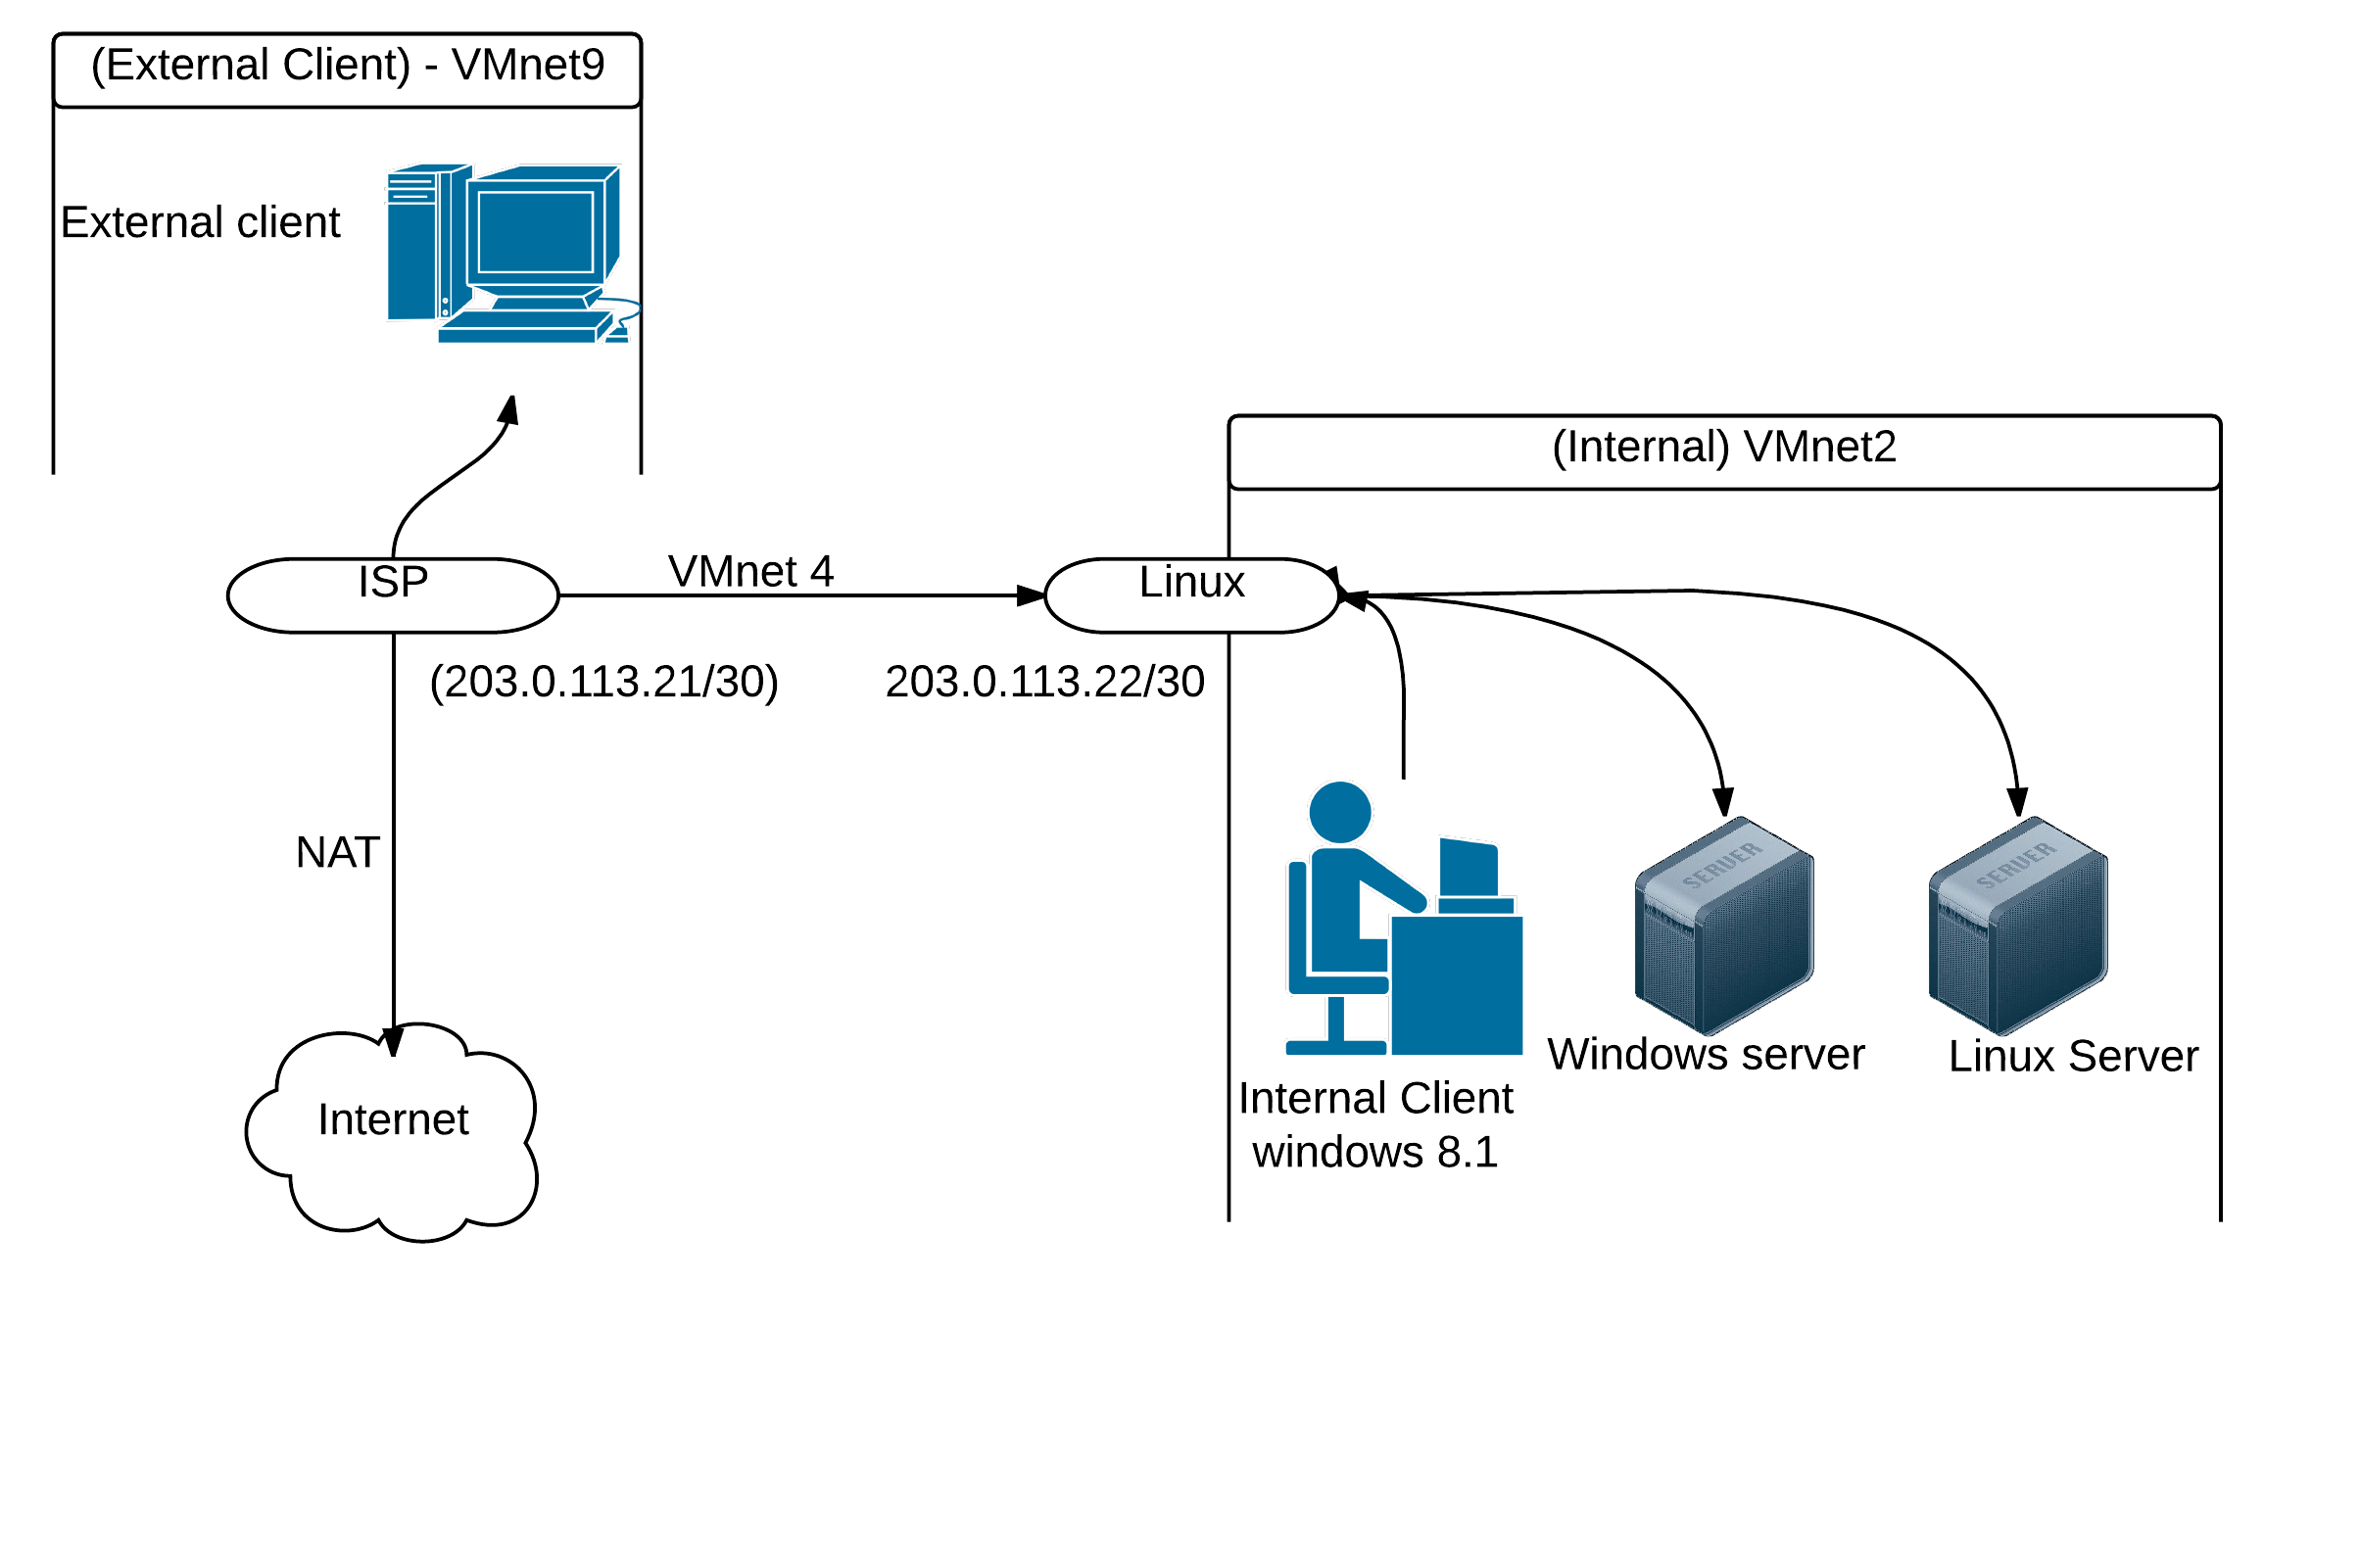
\includegraphics[width=1\linewidth]{./network}
\caption[Figur över nätverket i labb 1]{Nätverkets som ska sättas upp i Labb 1.}
\label{fig:network}
\end{figure}


Ni har fått i uppdrag att sätta upp ett nystartat företags nätverk. I \figurename  \ref{fig:network} ser ni hur nätverket ska se ut när ni är klara men labb 1.

Det är ett mycket enkelt nätverk ni ska sätta upp med en filserver och två klienter. För att komma ut på Internet så måste ni även sätta upp en server som agerar router mellan LANet och Internet.

\section{Krav}
\label{tasks}
Utöver nätverksskissen har ni fått en del krav som företaget har satta upp:

\begin{itemize}
    \item Alla maskiner ska:
    \begin{itemize}
        \item vara konfigurerade enligt nätverksskissen i \figurename \ref{fig:network}
        \item köra statisk IP-adressering, nätadresser får ni själva välja men motivera ert val i labbrapporten
        \item komma ut på Internet via routermaskinen
        \item ha Windows brandväggen påslagen
    \end{itemize}
    \item Man ska kunna pinga alla maskiners LAN nätverk
    \item Ni ska själva komma fram till vilka namn ni ska använda på era servrar och klienter, tänk på att motivera ert val i labbrapporten
    \item Klienterna \& filserven ska ha 4 lokala användarkonton: \\ \textit{OBS! För att utdelningarna ska fungerar så måste det vara samma lösenord på klienterna och serven för ett individuellt konto}
    \begin{itemize}
        \item Kalle Karlsson, användarnamn: \textbf{Kalle}
        \item Anna Johansson, användarnamn: \textbf{Anna}
        \item Stina Nilsson, användarnamn: \textbf{Stina}
        \item Johan Andersson, användarnamn: \textbf{Johan}
    \end{itemize}
    \item Specifika maskinkrav:
    \begin{itemize}
        \item \textbf{ISP Gateway}
        \begin{itemize}
            \item detta är den enda maskinen som ni inte installerar själva, det är en förkonfigurerad maskin som ni skapar en länkad klon av
            \item templaten finns här: \textbf{L:\textbackslash VirtualLabs\textbackslash Files\textbackslash Templates\textbackslash ISP Gateway Template\textbackslash }
        \end{itemize}

        \item \textbf{Routermaskinen}
        \begin{itemize}
            \item ska ha två nätverkskort, ett till LAN och ett till WAN
            \item WANet ska vara konfigurerat enligt nätverksskissen i \figurename \ref{fig:network}, \textit{OBS! För att kunna göra namnuppslag så måste man använda sig av ISP Gatwayens DNS server.}
            \item Ska användas som en form av webbproxy, detta uppnås genom att installerar rollen \textbf{Remote Access -> Routing}
            \item När rollen är installerad öppnar man upp MMCn för \textbf{Routing and Remote Access} och konfigurerar NAT mellan LANet och WANet
        \end{itemize}

        \item \textbf{Filserven}
        \begin{itemize}
            \item Följande tre lokala grupper ska finnas
            \begin{itemize}
                \item \textbf{All-Users} medlemmar: \textbf{Anna, Stina, Kalle \& Johan}
                \item \textbf{Accounting} medlemmar: \textbf{Anna, Stina \& Johan}
                \item \textbf{Sales} medlemmar: \textbf{Kalle, Stina \& Johan}
            \end{itemize}
            \item En extra hårddisk där de utdelade katalogerna ska placeras
            \item 7 utdelade kataloger: \\ \textit{OBS! \textbf{Administrator} och \textbf{System} ska alltid har fulla rättigheter till alla utdelningar}
            \begin{itemize}
                \item Namn: \textbf{Share}, rättigheter: \textbf{All-Users}(Läs/Skriv)
                \item Namn: \textbf{Accounting}, rättigheter: \textbf{Accounting}(Läs/Skriv)
                \item Namn: \textbf{Sales}, rättigheter: \textbf{Sales}(Läs/Skriv), \textbf{Accounting}(Läs)
                \item Namn: \textbf{Kalle}, rättigheter: \textbf{Kalle}(Läs/Skriv)
                \item Namn: \textbf{Anna}, rättigheter: \textbf{Anna}(Läs/Skriv)
                \item Namn: \textbf{Stina}, rättigheter: \textbf{Stina}(Läs/Skriv)
                \item Namn: \textbf{Johan}, rättigheter: \textbf{Johan}(Läs/Skriv)
            \end{itemize}
        \end{itemize}
    \end{itemize}
\end{itemize}

\section{Arbetsmiljö}
\label{enviroment}
Du kommer att använda VMware Workstation för att utföra denna labb. Du kommer endast att använda templates för ISP Gateway i den här labben resten du får själv skapa.

För att kunna kunna börja laborationen så måste du anmält dig till MSDNAA och en labbgrupp. När du gjort det så kan det ta upp till en arbetsdag innan du lagts till i systemen. 
\paragraph{Hjälpmedel} Till din hjälp så finns \win{2012 R2} och Windows 8.1 ISOs på 
L:\textbackslash VirtualLabs\textbackslash Files\textbackslash CD\textbackslash Microsoft\textbackslash 
\begin{itemize}
\item 9600.16384.WINBLUE\_RTM.130821-1623\_X64FRE\_SERVER\_EVAL\_EN-US-IRM\_SSS\_X64FREE\_EN-US\_DV5.ISO
\item 9600.16384.WINBLUE\_RTM.130821-1623\_X64FRE\_ENTERPRISE\_EVAL\_EN-US-IRM\_CENA\_X64FREE\_EN-US\_DV5.ISO
\end{itemize}
Windows 7 ISOn hittar du här: \textbf{L:\textbackslash VirtualLabs\textbackslash Files\textbackslash MSDNAA\textbackslash Operating Systems\textbackslash en\_windows\_7\_enterprise\_with\_sp1\_x64\_dvd\_620201.iso
}\end{document}
